% Drawing 156-8/01-2 -- folder 156-8, batch 01, archive page 10 (PDF page 11).
% Transcription: un segment gradué ; une accolade inférieure désigne le segment entier, $Z$ ; une accolade supérieure en désigne une partie, $Y$ ; un point marqué à l'extrémité de cette partie, désigné par une flèche, est $X$.
% Kind: segment with braces. Method 2 (schematic redraw from the facsimile). Status: ok.
% Notes: A graduated segment (three ticks), the lower brace Z over the whole, the upper brace Y over a part, the point X at the end of that part, shown by an arrow. The upper label sits on the bbox's top edge.
% Coordinates: 1 unit = 1 mm = 1/100 of the crop width (bbox in page fractions: [0.3, 0.585, 0.66, 0.66]).
% Redrawn by Claude (claude-opus-5-5), issue #73 pilot, 2026-11-07; not checked by a human; not compiled (no TeX in the session).
% Rights: reproduces part of the work -- behind RENDER_TRANSCRIPTS, never published by itself.
\documentclass[tikz,border=3pt]{standalone}
\usepackage{amsmath,amssymb}
\usetikzlibrary{patterns,arrows.meta}
\tikzset{pencil/.style={black!45}, struck/.style={black!35}, mark/.style={circle,draw,inner sep=1.3pt}, pt/.style={circle,fill,inner sep=0.9pt}, opt/.style={circle,draw,fill=white,inner sep=1.1pt}}
\begin{document}
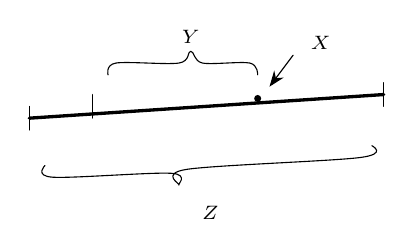
\begin{tikzpicture}[x=1mm,y=1mm,line cap=round,line join=round,font=\scriptsize]
\draw[very thick] (20,-11.5) -- (65,-8.5);
\draw (20,-10) -- (20,-13);
\draw (28,-8.5) -- (28,-11.5);
\draw (65,-7) -- (65,-10);
\node[pt] at (49,-9) {};
\draw plot[smooth, tension=0.55] coordinates {(30,-6) (31,-4.5) (39,-4.5) (40.5,-3) (42,-4.5) (48,-4.5) (49,-6)};
\node[inner sep=1pt] at (40.5,-1.2) {\scriptsize $Y$};
\draw[-{Stealth[length=2mm]}] (53.5,-3.5) -- (50.5,-7.5);
\node[inner sep=1pt] at (57,-2) {\scriptsize $X$};
\draw plot[smooth, tension=0.55] coordinates {(22,-17.5) (23,-19) (38,-18.5) (39,-20) (40,-18) (62,-16.5) (63.5,-15)};
\node[inner sep=1pt] at (43,-23.5) {\scriptsize $Z$};
\end{tikzpicture}
\end{document}
